
\documentclass[twocolumn, a4paper]{ieicejsp}
\usepackage{newenum}
\usepackage{comment}
\usepackage{ascmac}
\usepackage{amsmath}
\usepackage{amssymb}
\usepackage{amsfonts}
\usepackage[dvipdfmx]{graphicx}
\usepackage{multirow}
\usepackage{here}
\usepackage{bm}
\usepackage{epsfig}
\usepackage{array}

\newcommand{\fmusic}{f_{\mathrm{MUSIC}}}
\newcommand{\fprev}{f_{\mathrm{prev}}}
\newcommand{\fcurr}{f_{\mathrm{curr}}}

\title{MUSICアルゴリズムに基づく非接触型心拍数推定
  {\normalsize \\ Non-contact Heart Rate Estimation based on MUSIC Algorithm}}
  \author{
    山本幸平$^1$ \\ Kohei Yamamoto \and
    豊田健太郎$^2$\\ Kentaroh Toyoda \and
    大槻知明$^2$ \\ Tomoaki Ohtsuki \and
  }
 \affliate{
    慶應義塾大学大学院 理工学研究科$^1$ \\
    Graduate School of Science and Technology, Keio university \and
    慶應義塾大学 理工学部$^2$ \\    
    Faculty of Science and Technology, Keio university
}

\begin{document}
\maketitle

{\small
\section{はじめに}
心拍数推定は, ストレスを推定するための重要な技術の1つであり, 非接触性という特徴からドップラーセンサを用いた手法が様々提案されている.
FFT (Fourier Transform) に基づく手法が代表的であるが, MUSIC (MUltiple SIgnal Classification) アルゴリズムに基づく従来手法は, より高精度に心拍数を推定できることが示されている~[1].
しかしながら, この従来手法は解析信号を構成する正弦波の数 $P$ を推定する必要がある.
$P$を推定せずに心拍数を推定する手法も従来検討されているが~[2], 60~秒程度の長いウィンドウで1つの心拍数を推定するため, ストレス推定に必要な数秒程度の細かい心拍数変動を推定できないという問題がある.
そこで, 本稿では解析信号を複数の余弦波に分解し, 心拍に起因する成分のみを用いて信号を再構成することで $P$ を推定し, 短いウィンドウで心拍数を推定する手法を提案し, 実験を通して提案法と従来法の特性を比較評価する.
\vspace{-0.2cm}
\section{MUSIC アルゴリズム}

MUSIC アルゴリズムでは, 白色ガウス雑音存在下で解析信号が $P$ 個の正弦波から構成されていると仮定し, 周波数を推定する.
まず, 解析信号の共分散行列$R_x$を算出し, $R_x$を固有値分解する.
算出した固有値を降順に並べた場合, 最初の$P$個及び残りの$N-P$個の固有ベクトルにより信号空間と雑音空間がそれぞれ構成される.
ここで, $N$ は固有値の数である.
最終的に, MUSIC アルゴリズムにより算出されるスペクトル$\fmusic$は以下のように算出される.
\vspace{-0.2cm}
\begin{eqnarray}
  \fmusic(e^{j\omega}) = \frac{1}{\sum \limits_{i=P+1}^{N}|\bm{e}^H\bm{v}_i|^2},\\
  \bm{e} = [1, e^{j\omega}, e^{2j\omega}, e^{3j\omega}, ..., e^{(N-1)j\omega}]^T.
    \vspace{-0.2cm}
\end{eqnarray}
ここで, $\omega$ は角周波数, $\bm{v}_i$ は $i$ 番目の固有ベクトルである.

\vspace{-0.2cm}
\section{提案法}
提案法では, MUSIC アルゴリズムを用いる前に, 解析信号にDCT (Discrete Cosine Transform)を適用することで複数の余弦波に分解し, 心拍に起因する成分を抽出する.
そして, 抽出した成分のみを用いて IDCT (Inverse DCT) を行うことで, 信号を再構成する.
これにより, MUSICアルゴリズムで使用するパラメータ$P$を推定するとともに, 呼吸や体動に起因する雑音の影響を低減し, 短いウィンドウでも心拍数を推定できるようにする.
以下に, 提案法のアルゴリズムを示す.
\begin{enumerate}
%\item ドップラーセンサの受信信号Iデータ$I(T)$及びQデータ$Q(t)$を1000Hzから125Hzにダウンサンプリングする.
\item ウィンドウサイズ $W$ 及びステップサイズ $S$でIデータ$I(T)$及びQデータ$Q(t)$を取得し, 位相信号$\varphi(t)$を以下のように算出する.\\
\vspace{-0.5cm}
\begin{eqnarray}
  \varphi(t) = \arctan \frac{Q(t)}{I(t)}.
  \vspace{-0.2cm}
\end{eqnarray}
\vspace{-0.4cm}
\item 位相信号 $\varphi(t)$ に通過帯域が$[0.5,2]$ HzのBPF (Band Pass Filter) を適用する.
\item DCT をフィルタ後の位相信号 $\varphi(t)$ に適用する.
\item 1つ前のウィンドウで推定した心拍の基本周波数 $\fprev$ と現在のウィンドウで推定される周波数の最大変化量を$\Delta$として, 心拍の基本周波数及び第1高調波, 第2高調波に関連する可能性のある成分を, 周波数帯域 $[\fprev-\Delta, \fprev+\Delta]$~Hz 及び $[2(\fprev-\Delta),2(\fprev+\Delta)]$~Hz, $[3(\fprev-\Delta),3(\fprev+\Delta)]$~Hz からそれぞれ抽出する.
\item 抽出した成分に IDCT を適用し, 信号を再構成する.
\item 抽出した成分数を$P$として, MUSICアルゴリズムを再構成信号に適用し, スペクトル$\fmusic$を算出する.
\item $\fmusic$の最大ピーク検出に基づき, $\Delta$を用いて心拍に起因する周波数$\fcurr$を以下のように推定する.
\vspace{-0.1cm}
\begin{eqnarray}
  \fcurr = \begin{cases}
  	f' & {\rm if}~|f'-\fprev| \leq \Delta, \\
	\fprev & {\rm otherwise}.
  \end{cases}
\end{eqnarray}
ここで, $f'$は$\fmusic$の最大ピークが生じる周波数である.
\end{enumerate}

\vspace{-0.2cm}
\section{特性評価}

10人の被験者に対して, 着座静止及びタイピング時に120秒間心拍数を推定し, 心電図により算出した心拍数を真値として, 推定値と真値の絶対誤差を算出した.
提案法のウィンドウサイズ $W$ 及びステップサイズ $S$, $\Delta$ はそれぞれ 5~秒及び0.5~秒, 0.17~Hz とした.
図1に推定した心拍数変動の1例を示す.
図1より, 提案法は従来法~\cite{conv}と比較し, 例えば  30~秒から35~秒にかけての心拍変動のような, 5秒程度の細かい心拍数変動を高精度に推定できていることがわかる.
結果として, 提案法により, 着座静止及びタイピング時の従来法の平均絶対誤差が, それぞれ 48.8~\%及び 38.6~\% 改善された.
しかしながら, 実際の心拍変動が大きい被験者の場合, 心拍に起因するピークが複数生じるため, ピークを誤検出する場合も確認した.
そのため, 今後の研究ではピーク追跡法を検討することで, 推定精度をさらに改善する必要がある.

\begin{figure}[t]
\begin{center}
  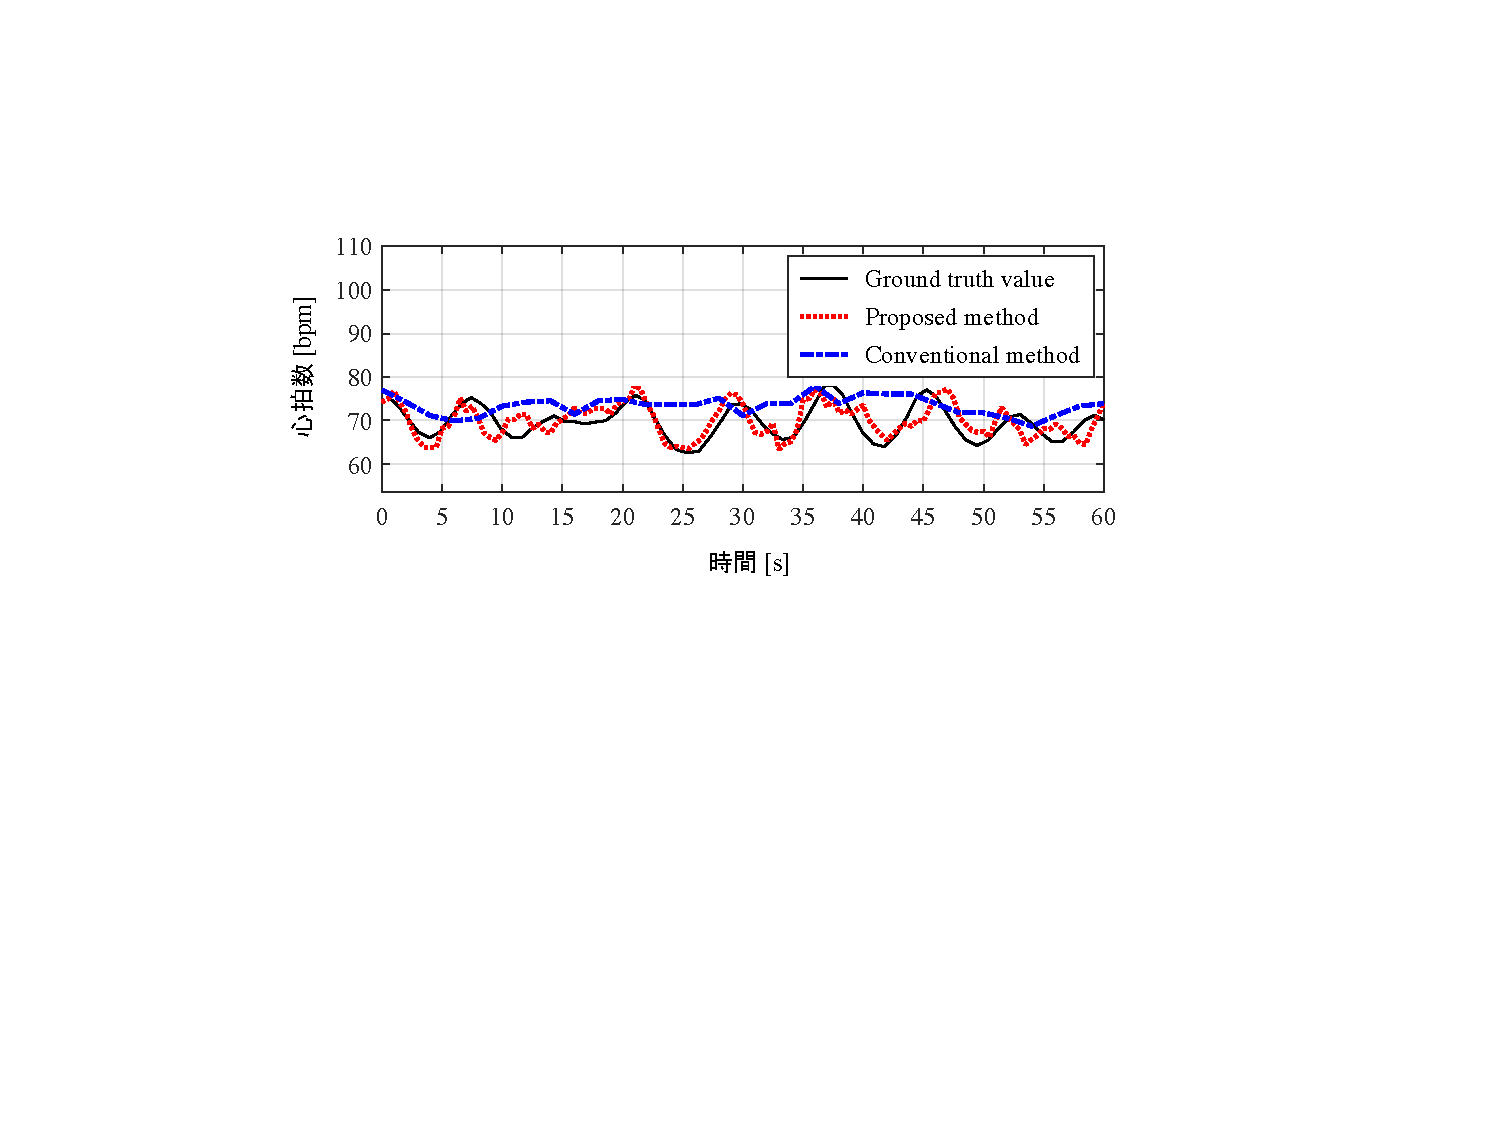
\includegraphics[width=7cm]{./HRvariation.pdf}
  \caption{{\small 推定した心拍数変動の1例.}}
  \label{fig:HRvariation}
 \end{center}
\end{figure}

\vspace{-0.2cm}
\section{おわりに}

本稿では,MUSIC アルゴリズムに基づく非接触型心拍数推定法を提案した. 
10 人の被験者に対する実験を通し, 提案法が従来法の平均AEを, 着座静止及びタイピング時のどちらの場合にも大きく改善することを確認した.


\vspace{-0.1cm}
%{\scriptsize
{\scriptsize
\begin{thebibliography}{9}

\bibitem{related} P. Bechet~\textit{et al.}, ``A non-contact method based on multiple signal classification algorithm to reduce the measurement time for accurately heart rate detection,'' {\it Review of Scientific Instruments}, vol. 84, Aug. 2013. 

\bibitem{conv} K. J. Lee~\textit{et al.}, ``Tracking driver's heart rate by continuous-wave Doppler radar,'' {\it EMBC}, pp. 5417-5420, Aug. 2016. 


\end{thebibliography}
}

\end{document}
